\documentclass[tikz,border=8pt]{standalone}
% Requer xelatex e a fonte Poppins. Ajuste o Path abaixo (ou use \setmainfont{Poppins} se ela estiver instalada).
\usepackage{fontspec}
\setmainfont{Poppins}[Path=/usr/share/fonts/truetype/google-fonts/,Extension=.ttf,UprightFont=*-Regular,BoldFont=*-Bold,ItalicFont=*-Italic,BoldItalicFont=*-BoldItalic]
\usepackage{xcolor}
\definecolor{azulescuro}{HTML}{4A6F9C}
\definecolor{azulmedio}{HTML}{6F93BC}
\definecolor{azulclaro}{HTML}{E9EDF3}
\definecolor{azulsenac}{HTML}{1F4E9A}
\definecolor{laranja}{HTML}{F19E37}
\definecolor{laranjaescuro}{HTML}{D9731A}
\definecolor{laranjaclaro}{HTML}{FDEFD9}
\definecolor{cinzatitulo}{HTML}{333333}
\definecolor{cinzatexto}{HTML}{5C5C5C}
\usepackage{tikz}
\usetikzlibrary{positioning,arrows.meta,fit,backgrounds,calc}

\definecolor{aresta}{HTML}{AEB8C6}
\begin{document}
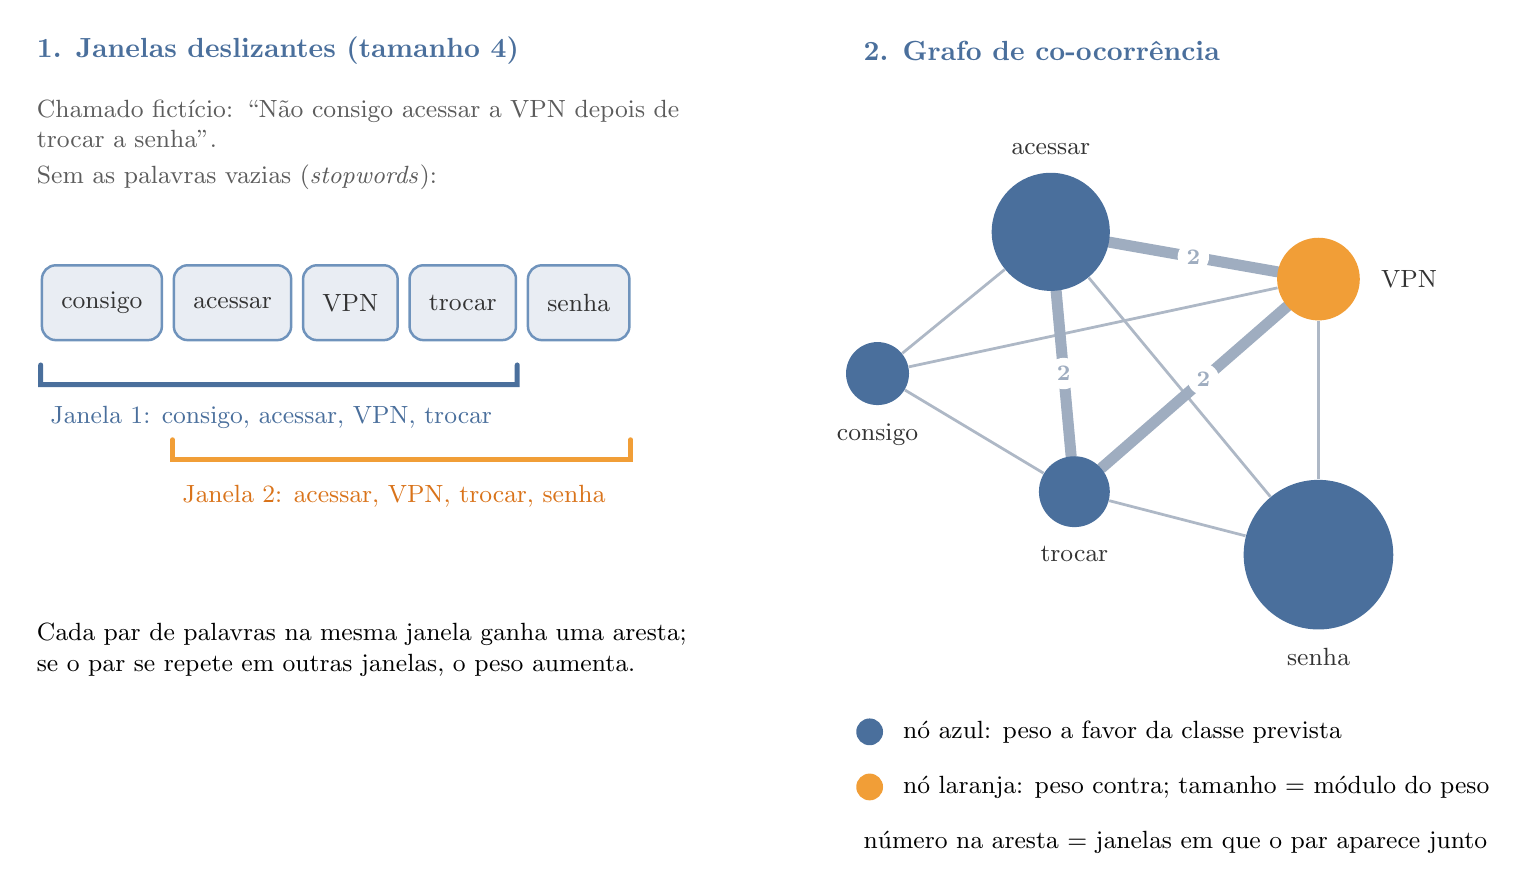
\begin{tikzpicture}[font=\small\color{cinzatexto},
  tit/.style={font=\normalsize\bfseries\color{azulescuro}, anchor=west},
  pal/.style={draw=azulmedio, fill=azulclaro, line width=0.9pt, rounded corners=5pt, minimum height=0.95cm, font=\small\color{cinzatitulo}, inner xsep=7pt},
  no/.style={circle, inner sep=0pt, text=cinzatitulo, font=\small\bfseries},
  e1/.style={aresta, line width=1pt},
  e2/.style={aresta!85!azulescuro, line width=4pt, line cap=round},
  num/.style={circle, fill=white, inner sep=1.5pt, font=\footnotesize\bfseries\color{cinzatitulo}}]
% ================= painel 1
\node[tit] at (0,6.6) {1. Janelas deslizantes (tamanho 4)};
\node[anchor=north west, text width=8.6cm, align=left] at (0,6.1) {\hyphenpenalty=10000 Chamado fictício: “Não consigo acessar a VPN depois de trocar a senha”.\\[2pt] Sem as palavras vazias (\textit{stopwords}):};
\node[pal] (p1) at (0.95,3.4) {consigo};
\node[pal, right=0.12cm of p1] (p2) {acessar};
\node[pal, right=0.12cm of p2] (p3) {VPN};
\node[pal, right=0.12cm of p3] (p4) {trocar};
\node[pal, right=0.12cm of p4] (p5) {senha};
% janela 1
\draw[azulescuro, line width=1.8pt, line cap=round] ($(p1.south west)+(0,-0.3)$) -- ++(0,-0.25) -- ($(p4.south east)+(0,-0.55)$) -- ++(0,0.25);
\node[anchor=north west, font=\small\color{azulescuro}] at ($(p1.south west)+(0,-0.7)$) {Janela 1: consigo, acessar, VPN, trocar};
% janela 2
\coordinate (w2a) at ($(p2.south west)+(0,-1.5)$);
\coordinate (w2b) at ($(p5.south east)+(0,-1.5)$);
\draw[laranja, line width=1.8pt, line cap=round] ($(w2a)+(0,0.25)$) -- (w2a) -- (w2b) -- ($(w2b)+(0,0.25)$);
\node[anchor=north west, font=\small\color{laranjaescuro}] at ($(w2a)+(0.0,-0.2)$) {Janela 2: acessar, VPN, trocar, senha};
\node[anchor=north west, text width=8.6cm, align=left, font=\small] at (0,-0.55) {\hyphenpenalty=10000 Cada par de palavras na mesma janela ganha uma aresta; se o par se repete em outras janelas, o peso aumenta.};
% ================= painel 2
\def\ox{10.8}
\node[tit] at (\ox-0.3,6.6) {2. Grafo de co-ocorrência};
\node[no, fill=azulescuro, minimum size=1.5cm] (acessar) at (\ox+2.2,4.3) {};
\node[no, fill=laranja, minimum size=1.05cm] (vpn) at (\ox+5.6,3.7) {};
\node[no, fill=azulescuro, minimum size=0.8cm] (consigo) at (\ox+0.0,2.5) {};
\node[no, fill=azulescuro, minimum size=0.9cm] (trocar) at (\ox+2.5,1.0) {};
\node[no, fill=azulescuro, minimum size=1.9cm] (senha) at (\ox+5.6,0.2) {};
\begin{scope}[on background layer]
\draw[e1] (consigo)--(acessar); \draw[e1] (consigo)--(vpn); \draw[e1] (consigo)--(trocar);
\draw[e1] (acessar)--(senha); \draw[e1] (vpn)--(senha); \draw[e1] (trocar)--(senha);
\draw[e2] (acessar)--(vpn) node[num, pos=0.5] {2};
\draw[e2] (acessar)--(trocar) node[num, pos=0.5] {2};
\draw[e2] (vpn)--(trocar) node[num, pos=0.45] {2};
\end{scope}
\node[above=3pt of acessar, font=\small\color{cinzatitulo}] {acessar};
\node[right=4pt of vpn, font=\small\color{cinzatitulo}] {VPN};
\node[below=3pt of consigo, font=\small\color{cinzatitulo}] {consigo};
\node[below=3pt of trocar, font=\small\color{cinzatitulo}] {trocar};
\node[below=3pt of senha, font=\small\color{cinzatitulo}] {senha};
% legenda
\fill[azulescuro] (\ox-0.1,-2.05) circle (0.17);
\node[anchor=west, font=\small] at (\ox+0.2,-2.05) {nó azul: peso a favor da classe prevista};
\fill[laranja] (\ox-0.1,-2.75) circle (0.17);
\node[anchor=west, font=\small] at (\ox+0.2,-2.75) {nó laranja: peso contra; tamanho = módulo do peso};
\node[anchor=west, font=\small] at (\ox-0.3,-3.45) {número na aresta = janelas em que o par aparece junto};
\end{tikzpicture}
\end{document}
